\documentclass{llncs}
\usepackage{epsfig,amsmath,graphicx,cite,lmodern}
\usepackage{subfig,svg}
\usepackage[utf8]{inputenc}

\begin{document}
\mainmatter

\title{Eine Übersicht über Crossover-Operationen für genetische Algorithmen\\Seminar Organic Computing}
\titlerunning{Eine Übersicht über Crossover-Operationen für genetische Algorithmen}  % abbreviated title (for running head)

\author{Gerald Siegert\\Matrikelnummer: 1450117}
\authorrunning{Siegert} % abbreviated author list (for running head)
\tocauthor{}

\institute{Universität Augsburg\\Lehrstuhl für Organic Computing\\
\email{student@organic-computing.org}}

\maketitle


%-------------------------
\begin{abstract}
	Zusammenfassung des Inhalts des Papers in ca. 200 Wörtern.
\end{abstract}

\pagebreak

\section{Einführung in genetische Algorithmen}
\label{sec:EinfuhrungGA}

	Genetische Algorithmen sind genauso wie andere Evolutionäre Algorithmen im Allgemeinen aus der Biologie übernommen worden. Wie der Name schon aussagt, basieren sie auf dem Prinzip der Evolution, bei der basierend auf einer Ausgangspopulation möglicher Lösungen neue Kinder erzeugt werden, welche dann die Vorfahren in der Population verdrängen. Welche Vorfahren, oder gar die erzeugten Kinder, dabei konkret verdrängt werden, entscheidet sich basierend auf einer Fitness-Funktion, bei der die gefundenen Lösungen der Population Evaluiert werden und anschließend die nur die besten in der Population verweilen dürfen.
	
	\begin{figure}
		\centering
		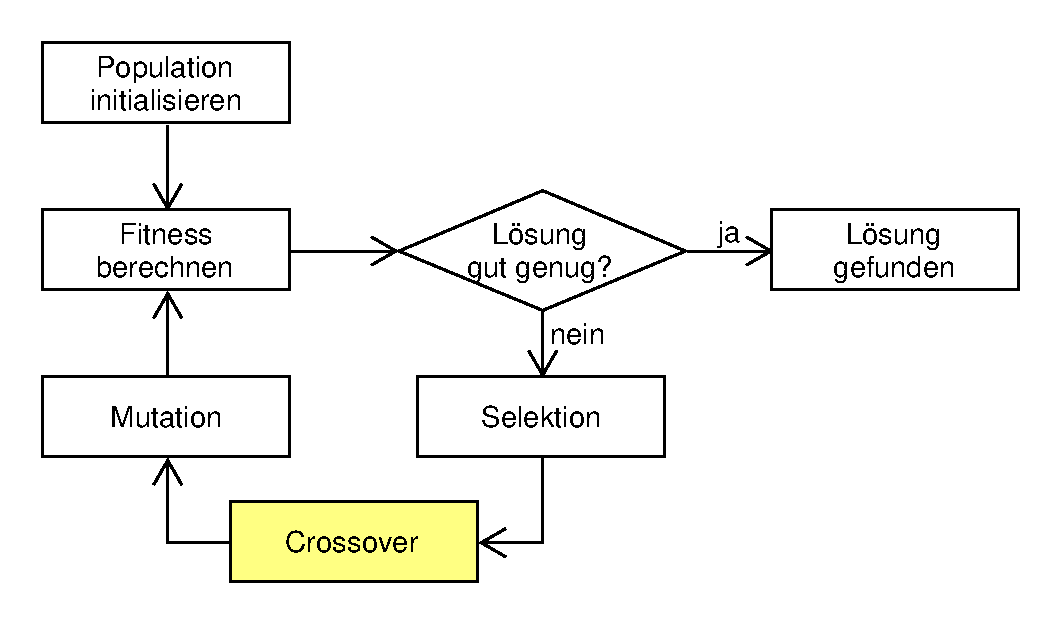
\includegraphics[width=.8\columnwidth]{./Figures/GA-Prinzip.pdf}
		\caption{Grundlegender Ablauf eines genetischen Algorithmus}
		\label{fig:abb1}
	\end{figure}	

	Die wichtigen Parameter eines GA selbst sind zum einen die Selektion der Gene, deren Crossover zur Erzeugung neuer Kinder, sowie die Durchführung anschließender Mutationen. Maßgeblich für die Qualität und Effizienz eines GA ist dabei die in Fig. \ref{fig:abb1} markierte Crossover-Operation. In dieser Seminararbeit soll daher nun ein kleiner Überblick über verschiedene Crossover-Operationen gegeben werden.

\section{Klassifizierungen von Crossover-Operationen}
\label{sec:KlassifizierungCrossover}

Klassifizierung von Crossover

\section{Eindimensionale Repräsentation}
\label{sec:EindimensionaleRep}

Eindimensionales

\subsection{Binäre Codierung}
\label{sec:BinCod}

Binär

\subsection{Codierung als Ganzzahlen}
\label{sec:IntCod}

Integer

\subsubsection{Operationen für ganzzahlige Werte}
\label{sec:IntOp}

Integer, die nicht als Binär gehandhabt werden

\subsubsection{Operationen für Permutationen}
\label{sec:PermOp}

Permutationen von Integer-Werten (zB TSP)

\subsection{Codierung als Fließkommazahl}
\label{sec:FloatCod}

Fließkommazahlen

\subsection{Codierung als Zeichenkette}
\label{sec:StrCod}

String-Codierungen

\section{Mehrdimensionale Repräsentation}
\label{sec:MehrdimRep}

Mehrdimensionale

\subsection{Codierung als Baum}
\label{sec:BaumCod}

Bäume und deren nutzen

\subsection{Codierung als Array}
\label{sec:ArrayCod}

Array und deren Nutzen

\subsection{Weitere Codierungen für mehrdimensionale Daten}
\label{sec:WeitereMehrdimensionale}

Kurz weiteres wie Matrizen und modularisierte Codierung

\section{Anwendungsspezifische Codierung der Daten}
\label{sec:AnwendungsspezifischeCod}

Kurz anwendungsspezifisches

\section{Universale Crossover-Operationen}
\label{sec:UniversaleOp}

Kurz auf weitere, universal einsetzbare Operationen eingehen (besser am Anfang?)

\section{Zusammenfassung und Ausblick}
\label{sec:Zusammenfassung}

Kurze Zusammenfassung

\bibliographystyle{splncs03} 
\bibliography{literature}





\newpage

%-------------------------
\section{Motivation}
\label{sec:Motivation}
Einführung ins Thema. Was bestehen für Probleme, wie soll das gelöst werden? \\

Wieso braucht man vorgestellte Technik/System/Algorithmus?



%-------------------------
\section{Stand der Technik} \label{sec:sdt}
%
Wie andere Verfahren das Problem zu lösen versuchen. \cite{OCBible}

%-------------------------
\section{Hauptteil}
\label{sec:Hauptteil}

\subsection{Grundlagen}
\label{sec:Grundlagen}
Text zu Fig.~\ref{fig:abb1}. Siehe Formel~\ref{eq:mean}

\subsubsection{Advantages and Challenges}
Eine Subsubsection.


\begin{figure}
	\centering
	\subfloat[Beispielbild 1]{
\includegraphics[width=0.5\columnwidth]{./Figures/Organic-Computing.png}}
	\hfill
	\subfloat[Beispielbild 2]{
\includegraphics[width=0.5\columnwidth]{./Figures/Organic-Computing.png}}
	\caption{Zwei Beispielbilder.}
\end{figure}

\begin{equation}
\label{eq:mean}
\bar{e} = \frac{1}{N}\sum_{i=1}^N{\lvert f_i - x_i\rvert}
\end{equation}


%-------------------------
\section{Evaluation}



\end{document}
